
%(BEGIN_QUESTION)
% Copyright 2011, Tony R. Kuphaldt, released under the Creative Commons Attribution License (v 1.0)
% This means you may do almost anything with this work of mine, so long as you give me proper credit

A process uses two split-ranged control valves (FV-82a and FV-82b, with ``progressive'' ranges) to control the flow of hydrogen gas entering a chemical reactor.  Valve (FV-82a) is the first of the two hydrogen valves to open (wide-open when FC-82's output is 50\%), while valve FV-82b is the last to open (just beginning to open when FC-82's output is 50\%).  The graphic display on the DCS is supposed to provide operators with a visual indication of the process, the proportion controller, and both valve positions:

$$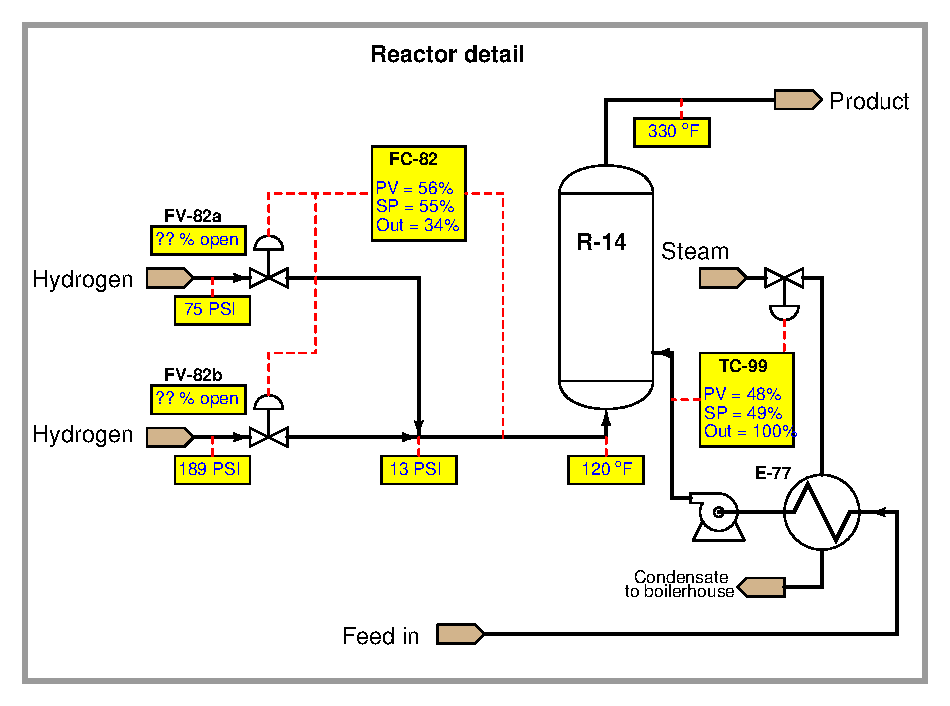
\includegraphics[width=15.5cm]{i01521x01.eps}$$

This graphic display, however, is not complete.  The engineer forgot to program it to display the individual positions of valves FV-82a and FV-82b.  The way it stands right now, the operator can see the controller's output signal (shown here at 34\%), but cannot tell what the individual stem positions are for each of the two split-ranged valves.  This task has been left to you!

\vskip 10pt

Write a formula for calculating each valve's position based on the output value from controller FC-82.  These formulae will be entered into the DCS to provide a display to the operator of each valve's stem position.  You may refer to the controller's output signal value as $x$ in each formula if you prefer:

\vskip 10pt

Position of valve FV-82a = 

\vskip 10pt

Position of valve FV-82b = 

\vskip 10pt

Don't worry about limiting these calculated values to prevent nonsense numbers like $<$ 0\% and $>$ 100\%, because this value-limiting can be easily programmed into the DCS display software.  Just write mathematical formulae to properly predict the two valve positions within their normal ranges.

\underbar{file i01521}
%(END_QUESTION)





%(BEGIN_ANSWER)

Position of valve FV-82a = {\tt (FC-82 Output) * 2}

\vskip 10pt

Position of valve FV-82b =  {\tt ((FC-82 Output) * 2) - 100}


%(END_ANSWER)





%(BEGIN_NOTES)

$$\includegraphics[width=15.5cm]{i01521x02.eps}$$

\vskip 20pt \vbox{\hrule \hbox{\strut \vrule{} {\bf Virtual Troubleshooting} \vrule} \hrule}

This question is a good candidate for a ``Virtual Troubleshooting'' exercise.  Presenting the diagram to students, you first imagine in your own mind a particular fault in the system.  Then, you present one or more symptoms of that fault (something noticeable by an operator or other user of the system).  Students then propose various diagnostic tests to perform on this system to identify the nature and location of the fault, as though they were technicians trying to troubleshoot the problem.  Your job is to tell them what the result(s) would be for each of the proposed diagnostic tests, documenting those results where all the students can see.

During and after the exercise, it is good to ask students follow-up questions such as:

\begin{itemize}
\item{} What does the result of the last diagnostic test tell you about the fault?
\item{} Suppose the results of the last diagnostic test were different.  What then would that result tell you about the fault?
\item{} Is the last diagnostic test the best one we could do?
\item{} What would be the ideal order of tests, to diagnose the problem in as few steps as possible?
\end{itemize}


%INDEX% Final Control Elements, valve: split ranging

%(END_NOTES)


